\chapter{Introduction to Dark Matter}
\label{chap:chap1}

%% Restart the numbering to make sure that this is definitely page #1!
\pagenumbering{arabic}

%%-----Chapter quote
\chapterquote{Place holder.}%
{Place holder, xxxx--xxxx}%: Blaa

Ever since humankind harnessed the capacity for curiosity, the universe, along with everything it holds has become a vast playground in which the game is to look outwards into the depths of the universe and inwards into the depths of the fabric, the fundamental building blocks of the universe. The introduction of general relativity, followed by the observations of Edwin Hubble lead to a picture of the universe that's non-static and ever expanding. Soon after, dynamical studies of galaxies and galaxy clusters by Fritz Zwicky unfolded a discrepancy between the expected luminous mass and inferred mass of such clusters \cite{Fritz_Zwicky_1993}. The presence of "dark" or unseen matter in galaxies was suggested by a variety of different techniques thereafter. Although unseen, the gravitational influence of dark matter is apparent in many facets of cosmology, leading to a universe that's predominantly dark in matter density and undiscovered. This chapter will explore the theoretical and observational motivations for dark matter, delving into the different candidates to explain it's nature and introducing the Weakly Interacting Massive Particles, one of the leading candidates for dark matter. 

\newpage

%%------------------------------$$
\section{Modern Cosmology}
\label{sec:moderncosmology}

Our modern understanding of the universe emerged with key cosmological observations and realisations at the start of the 20th century. The measurement of the first Doppler shift of the Andromeda galaxy in 1913 and the subsequent measurements made by Vesto Slipher, although controversial at the time, showed that almost all such galaxies were receding from Earth \cite{Slipler}. The expanding universe hypothesis was further strengthened by Georges Lemaître and Alexander Friedmann in the 1920s when they independently used Einstein's field equations to showed that the universe may be expanding \cite{Friedman}. But this hypothesis gained most of it's attraction when Erwin Hubble that showed the correlation between distant galaxies and their recession velocities---dubbed as Hubble's Law \cite{Hubble}.


%%----------------$$
\subsection{The Expanding Universe}

The spectral light from distant stars in galaxies outside of our local group appear to be shifted as these galaxies move away from Earth. Interpreted as the Doppler effect in flat spacetime, the velocity $v$ related to the shift in  spectral wavelength $\Delta \lambda/\lambda$ is given by the Doppler formula,
%
\begin{equation}
  v/c = \Delta \lambda/\lambda \equiv z,
\end{equation}
%
for $V \ll c$, where $z$ is the astronomical definition of redshift. 

Erwin Hubble showed that for galaxies sufficiently close, where their distance can be measured, the velocity $\vec{v}$ of these galaxies and their distance $\vec{r}$ followed a simple linear relationship, called Hubble's law:
%
\begin{equation}
  \boldsymbol{\vec{v}} = H_0\boldsymbol{\vec{r}}.
\end{equation}
%
The constant of proportionality, $H_0$ is called the Hubble constant. The Hubble constant represents the present day expansion rate of the universe and is usually given with a dimensionless parameter $h_0$, where
%
\begin{equation}\label{eq:hubble_constant}
  H_0 = 100h_0 \; \MathText{km} \; \MathText{s}^{-1} \; \MathText{Mpc}^{-1}, \; \MathText{where} \; h_0 = 0.674 \pm 0.005 \: \cite{Plank_2018}.
\end{equation}
%

Hubble's law is a phenomenological relationship between redshift and distance, implying that the further a galaxy is, the faster it is moving away from us. The law holds for galaxies that are far enough away that any velocity disruptions due to local gravitational effects are subdominant to the expansion rate. While at the same, these galaxies cannot be too far away that the effects of spacetime curvature or the expansion of the universe in the time it takes for the photons to travel become significant. 

The expansion of the universe leads to the concept of the expansion of space. The expansion is often represented in co-moving coordinates $\boldsymbol{\vec{x}}$. The distance associated with the expansion---the co-moving distance---is a time independent measure between two fundamental observers. In a universe that's expanding under isotropy and homogeneity, the physical distance or proper distance $\boldsymbol{\vec{r}}$ is related to the co-moving coordinates moving along with the expansion of space by
%
\begin{equation}
  \boldsymbol{\vec{r}} = a(t)\boldsymbol{\vec{x}},
\end{equation}
%
where $a(t)$ is the time-dependent cosmological scale factor, representing the change in distance between two fundamental observers due to the expansion.

Differentiating $\boldsymbol{\vec{r}}$ with respect to time leads to the recession velocity $\boldsymbol{\vec{v}}$ of an observer or a galaxy in the same direction as its displacement away from earth, where
%
\begin{equation}
  \boldsymbol{\vec{v}} = \dv{\boldsymbol{\vec{r}}}{t} \equiv  \dot{a(t)}\boldsymbol{\vec{x}},
\end{equation}
%
leading to the relationship,
%
\begin{equation}
  H(t) = \frac{\dot{a(t)}}{a(t)}.
\end{equation}
%
The equation above gives the connection of the Hubble constant to the geometry of spacetime, where $H(t)$ is the time-dependent Hubble parameter, defining the relative expansion of space. The Hubble constant $H_0$ we measure is $H(t)$ at the present time of the universe.

The expansion of space requires a time-dependent geometry in which a particle's energy moving through this geometry will change similar to it moving through a time-dependent potential. A photon whose energy is proportional to frequency and therefore its wavelength, will experience the expansion as a stretch in its wavelength. This cosmological redshift is defined in terms of the scale factor as
%
\begin{equation}
  z \equiv \frac{\lambda(t_0) - \lambda(t)}{\lambda(t)} = \frac{\lambda(t_0)}{\lambda(t)} -1 = \frac{a(t_0)}{a(t)} - 1,
\end{equation}
%
where $t$ represents cosmic time and $t_0$ present time.

The Hubble constant has the dimensions of an inverse time. The inversion is called the Hubble time $t_H$. In a version of the universe in which $\ddot{a(t)} \leq 0$, the Hubble time becomes an upper bound and a rough estimate of the age of the universe, placing the age to $\sim$ 14 billion years. With the cosmological observations of this era, the picture of the universe moved towards one in which the universe had a beginning and from that start came the expansion. But the Hubble expansion alone does not provide sufficient evidence and description for what is generally refer to as the hot Big Bang model of cosmology. The description comes from the application of the cosmological principle to Einstein's theory of General Relativity.

%%----------------$$
\subsection{Cosmological Principle}
\label{subsec:cosmological_principle}

The dynamics of the universe are governed by the Einstein field equation, relating the curvature of spacetime to density of mass-energy \cite{Gravity}
%
\begin{equation}\label{eq:einstein_field_eq}
  R_{\mu\nu} - \frac{1}{2} g_{\mu\nu}R + g_{\mu\nu}\Lambda = \frac{8\pi{}G}{c^4} T_{\mu\nu},
\end{equation}
%
where $R_{\mu\nu}$ is the Ricci curvature tensor, R is the scalar curvature, $g_{\mu\nu}$ is the metric tensor, $\lambda$ is the cosmological constant, $G$ is gravitational coupling constant and $T_{\mu\nu}$ is the stress–energy tensor. The left hand side of this equation describes the geometrical structure of spacetime and the right describes the measure of matter and energy density of the Universe. The cosmological constant $\Lambda$ was originally introduced by Einstein as a tuning mechanism for a static cosmology with non-zero matter content but later interpreted as the energy density of the vacuum, a source of energy and momentum that may be present in the absence of matter fields \cite{SeanC}.

Modern cosmology for some time has relied upon the premise offered by the cosmological principle. This principle states that the Universe on large scales is homogeneous and isotropic, where local variations in density are averaged over. A homogeneous, isotropic spacetime is one for which the geometry is spherically symmetric about any one point (isotropic) and the same in all points (homogeneous). Although isotropy and homogeneity is assumed for space, when we look at distant galaxies, they appear to be receding from us; the universe is apparently not static, but changing with time. Therefore, any cosmological model of the universe must assume a homogeneous and isotropic universe in space but not in time. Spacetime can therefore be considered as $\boldsymbol{T} \cross U$, where $\boldsymbol{T}$ represents the time direction and $U$ is a homogeneous and isotropic three-manifold. The usefulness of homogeneity and isotropy is that they imply that $U$ must be a maximally symmetric space, taking the form of a metric
%
\begin{equation}
    ds^2 = -dt^2 + a^2(t)\gamma_{ij}(u)du^2du^j,  
\end{equation}
%
where $t$ is the timelike coordinates, ($u^1, u^2, u^3$) are the coordinates on $U$ and $\gamma_{ij}$ is the maximally symmetric metric on $U$. The dimensionless scale factor $a(t)$ is a function of proper time $t$, representing the scale of the space-like slice of spacetime at the present moment.

The geometrical interpretation of the cosmological principle can be shown to take a similar form to that of equation (\ref{eq:einstein_field_eq}) as the Friedmann-Robertson-Walker (FRW) metric---a metric tensor which describes a homogeneous and isotropic spacetime that evolves as a function of time (see \cite{Modern_Cosmology, Gravity} for an in-depth review). The three line elements of the metric tensor can be written in a unified form to give the well known FRW metric,
%
\begin{equation}
  ds^2 = -dt^2 + a^2(t) \left[ \frac{dr^2}{1 - kr^2} +r^2(d\theta^2 + sin^2\theta d\phi) \right],
\end{equation}
%
where \textit{r}, \theta and \phi represent the co-moving polar coordinates. The parameter \textit{k} represents the curvature of the universe, where +1, 0, -1 is for a closed, flat or an open universe respectively, corresponding to a positive, zero or a negative curvature of space.

The FRW model assumes a cosmological fluid consisting of three non-interacting components: pressureless matter, relativistic particles \& radiation and vacuum. This can be modelled by an energy-momentum tensor of a perfect fluid, specified by an energy density $\rho$  and isotropic pressure $p$ as 
%
\begin{equation}\label{eq:em_tensor}
  T_{\mu\nu} = (\rho + p)u_{\mu}u_{\nu} + pg_{\mu\nu}, 
\end{equation}
%
where $u^{\mu}$ is the fluid four-momentum. Under the boundaries imposed by the cosmological principle, whereby the energy-momentum tensor takes the form of a perfect fluid (\ref{eq:em_tensor}), the Einstein field equation (\ref{eq:einstein_field_eq}) reduces to the Friedmann equations \cite{Friedman, SeanC}:
%
\begin{equation}
  H^2 \equiv \left( \frac{\dot{a}}{a} \right)^2 = \frac{8\pi{}G}{3}\rho - \frac{kc^2}{a^2} + \frac{\Lambda}{3}
\end{equation}
%
%
\begin{equation}\label{eq:friedmann_2}
    \frac{\ddot{a}}{a} = -\frac{4\pi{}G}{3}(\rho + 3p) + \frac{\Lambda{}c^2}{3}.
\end{equation}
%
Examining these equations under certain assumptions can lead to useful cosmological quantities. In assuming a flat spacetime, where spatial curvature $k=0$ and one which is static ($\Lambda = 0$), leads to the quantity known as the critical density, 
%
\begin{equation}\label{eq:crit_density}
  \rho_{crit} \equiv \frac{3H^2(t)}{8\pi{}G} \simeq 1.88 \times 10^{-29} \: h^2 \: \MathText{g cm}^{-3} \: \cite{pdg}.
\end{equation}
%
The cosmological density parameter, a useful definition in comparing different cosmological models is then defined as
%
\begin{equation}\label{eq:omega_tot}
  \Omega_{tot} = \frac{8\pi{}G}{3H^2}\rho = \frac{\rho}{\rho_{crit}}.
\end{equation}
%
Under the conditions where $\Lambda = 0$ and by using (\ref{eq:omega_tot}), the Friedmann equation (1.12) can be shown to take the form
%
\begin{equation}\label{eq:density_param}
  \Omega_{tot} - 1 = \frac{kc^2}{a^2H^2}, 
\end{equation}
%
where the sign of spacetime curvature parameter $k$ is determined by whether $\Omega_{tot}$ is greater than, equal to, or less than one. This reduction leads to a picture in which $\rho < \rho_{crit}$, $\rho = \rho_{crit}$ and $\rho > \rho_{crit}$, equate to a universe that is respectively open ($k=-1$), flat ($k=0$) or closed ($k=+1$). 

The observational determination of the density parameter is an area of intense investigation and it is often necessary to distinguish different contributions to the overall density. One can conveniently define the present-day density parameters for pressureless matter as $\Omega_{m}$, relativistic particles and radiation as $\Omega_r$ and the quantity $\Omega_{\Lambda} = \Lambda/3H^2$. Thus, the total density of the universe may be defined as, 
%
\begin{equation}
  \Omega_{tot} = \Omega_{r} + \Omega_{m} + \Omega_{\Lambda}. 
\end{equation}
%
The Friedmann equation then takes the form
%
\begin{equation}
  \frac{kc^2}{a_{0}^2H_{0}^2} = \Omega_{r} + \Omega_{m} + \Omega_{\Lambda} - 1
\end{equation}
%
where the subscript 0 indicates present day values. 

The conclusion one takes is that the curvature of space denoted by the left side of the equation depends on the sum of densities in matter, relativistic particles, and vacuum.  The $\Omega_{tot}$ parameter as given in (\ref{eq:density_param}), plays an important role in the evolution of universe through its gravitational potential. The observational determination of the density parameter and its constituents will highlight which of the three Robertson-Walker geometries describes our universe. In a simplified scenario in which $\Lambda = 0$ and universe is filled with fluids of positive energy ($\rho > 0$) and non-negative pressure ($p \geq 0$), equation (\ref{eq:friedmann_2}) leads to $\ddot{a} < 0$. Since the expansion of the universe is verified by the motion of distant galaxies, where $\dot{a} > 0$, this leads to the conclusion that the rate at which the universe is expanding is negative, hence the expansion is decelerating. This is as expected, since the gravitational attraction of the matter content of the universe works against expansion. In tracing the evolution backwards in time, a singularity is reached at $a = 0$. If $\ddot{a}$ were exactly zero, the age of the universe would be $H_{0}^{-1}$. The singularity represents a point in which the universe began from a singular state and this point in history is commonly known as the "big bang".  


%%------------------------------$$
\section{Evidence for Dark Matter}
\label{sec:darkmatter}

The evolution of the universe is governed by the total density content and from which, the interplay between the matter, radiation and vacuum densities. The cosmic inflation theory requires a universe that is flat, hence $\Omega_{tot} = 1$. With the premise that the universe is flat and by taking into account complementary theoretical and experimental techniques, it becomes possible to quantify the matter density of the universe. By examining the universe on  different cosmological scales via Big Bang Nucleosynthesis (BBN), the Cosmic Microwave Background (CMB) and Gravitational Lensing, a picture emerges in one which roughly 95\% of the total energy density of the universe still lacks scientific exploration and largely remains a mystery. This section will examine some of the leading cosmological and astronomical observations in more detail, concluding that the levels of observed or luminous matter in the universe does not account for the total matter and that the majority of the matter content of the universe is non-baryonic and non-luminous luminous. 

\subsection{Cosmic Microwave Background}
\label{subsec:CMB}

The cosmic microwave background radiation, first discovered in mid-1960s \cite{CMB_disc}, is thought of as a primordial radiation from the early universe. In the hot Big Bang model, the early universe is extremely hot and dense, leading to a constant scattering of particles and radiation. At around a redshift ~1100 and roughly 380,000 years of age, the expansion of space cooled the plasma, allowing the first atoms to form through recombination, effectively decoupling the radiation from matter and making the universe transparent to photons. The collisions of these photons with electrons before last scattering ensures that the photons were in equilibrium. Travelling freely through space, this radiation is still present today but has been redshifted due to the expansion of the universe. The CMB photons are detected on earth with a spectral distribution that of a black body function with $T = 2.725$ K \cite{cmb_temp}. The CMB as observed from earth is roughly homogeneous and isotropic but at scales of around $10^{-6}$, it contains small temperature fluctuations (or anisotropies). The most detailed observation to-date of the CMB anisotropies comes from the Planck collaboration \cite{plank_cmb_map}, where an all sky map of the temperature anisotropies measured by their space observatory is shown in figure (\ref{fig:cmb_map}).

\begin{figure}[ht!]
    \begin{center}
        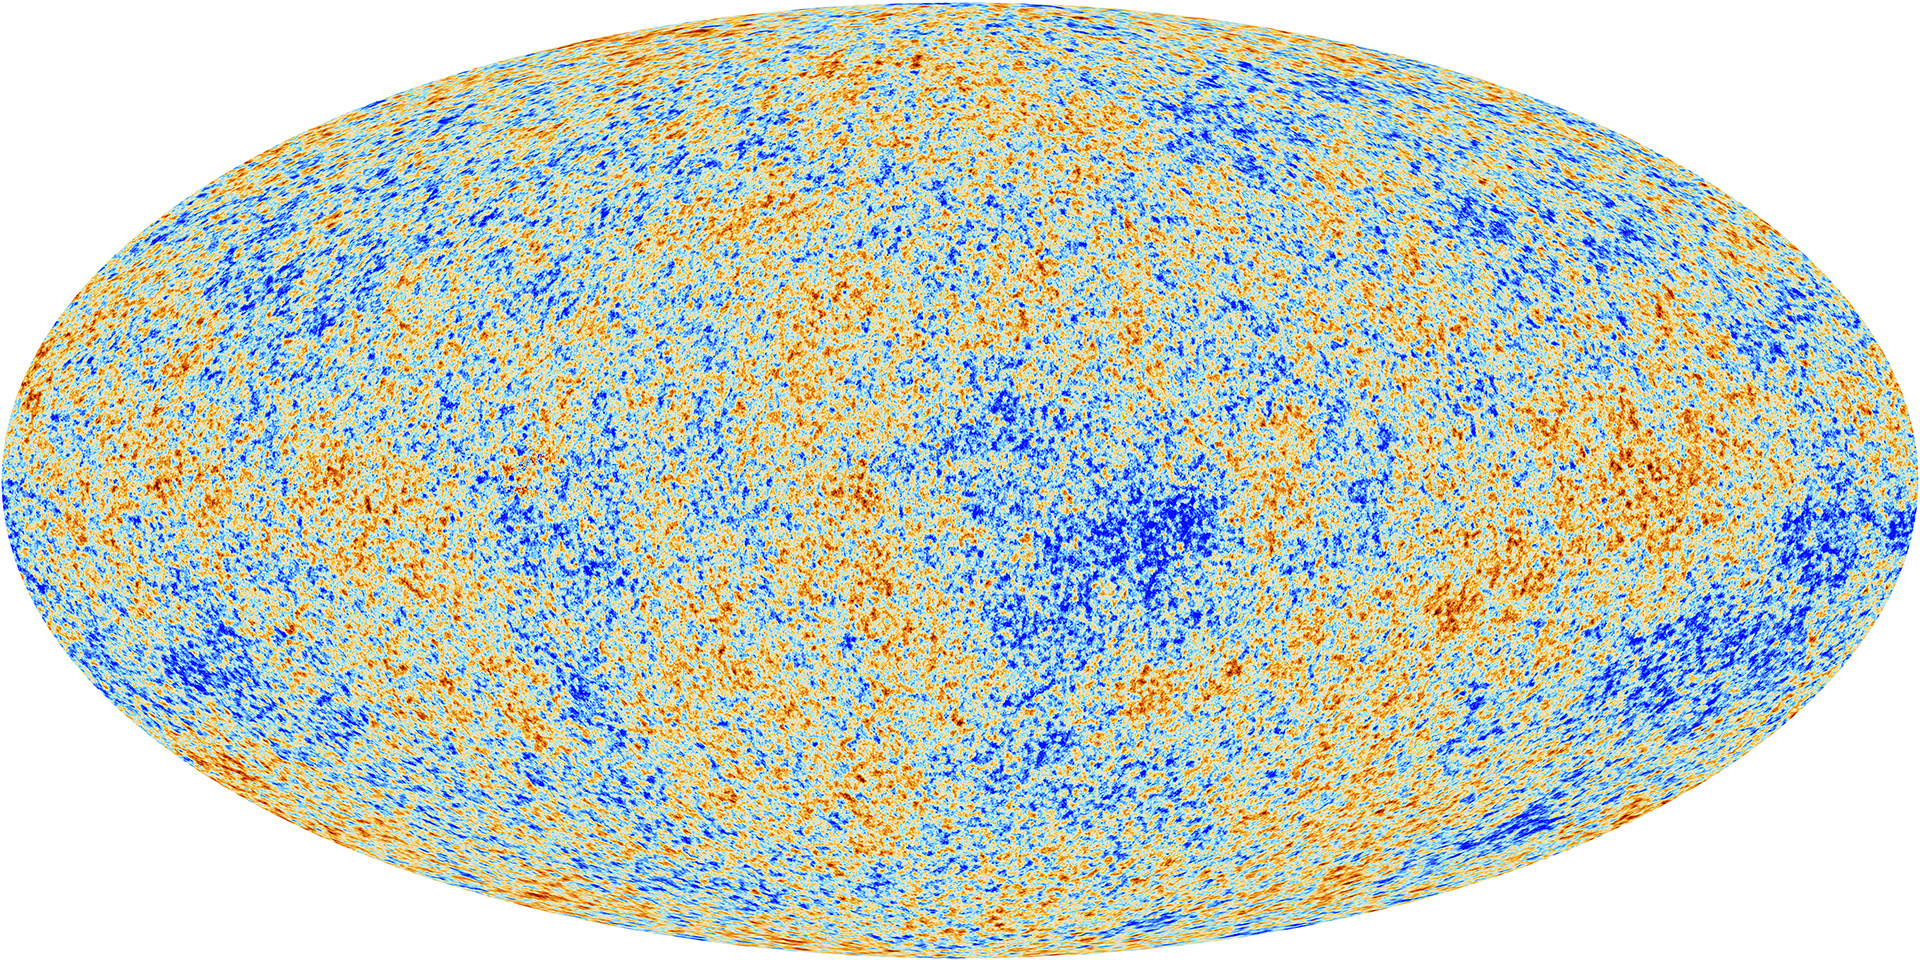
\includegraphics[scale=0.2]{Chapter_1/Figures/Planck_CMB.jpg}
        \caption[The map of the all sky CMB radiation as illustrated by the Planck collaboration, showing in detail the temperature anisotropies.]%
        {The map of the all sky CMB radiation as illustrated by the Planck collaboration, showing in detail the temperature anisotropies. The temperature difference between blue and red in the figure is a few thousandths of a Kelvin and correspond to matter density fluctuations in the distribution.}
        \label{fig:cmb_map}
        \end{center}
\end{figure}

The anisotropies observed in the CMB can be mapped at different angular scales. These angular scales are representations of the physical size of anisotropies at the time of the last-scatter. The angular scales of the fluctuations can be parametrised as the multipole moments ($l$) of a spherical harmonic, which determines the wavelength, $\lambda = 180\circ/l$ of the mode on the sphere of the CMB. The mapping of the different scales are given as the power spectrum of the CMB and shown in figure (\ref{fig:cmb_power_spectrum}).

\begin{figure}[ht!]
    \begin{center}
        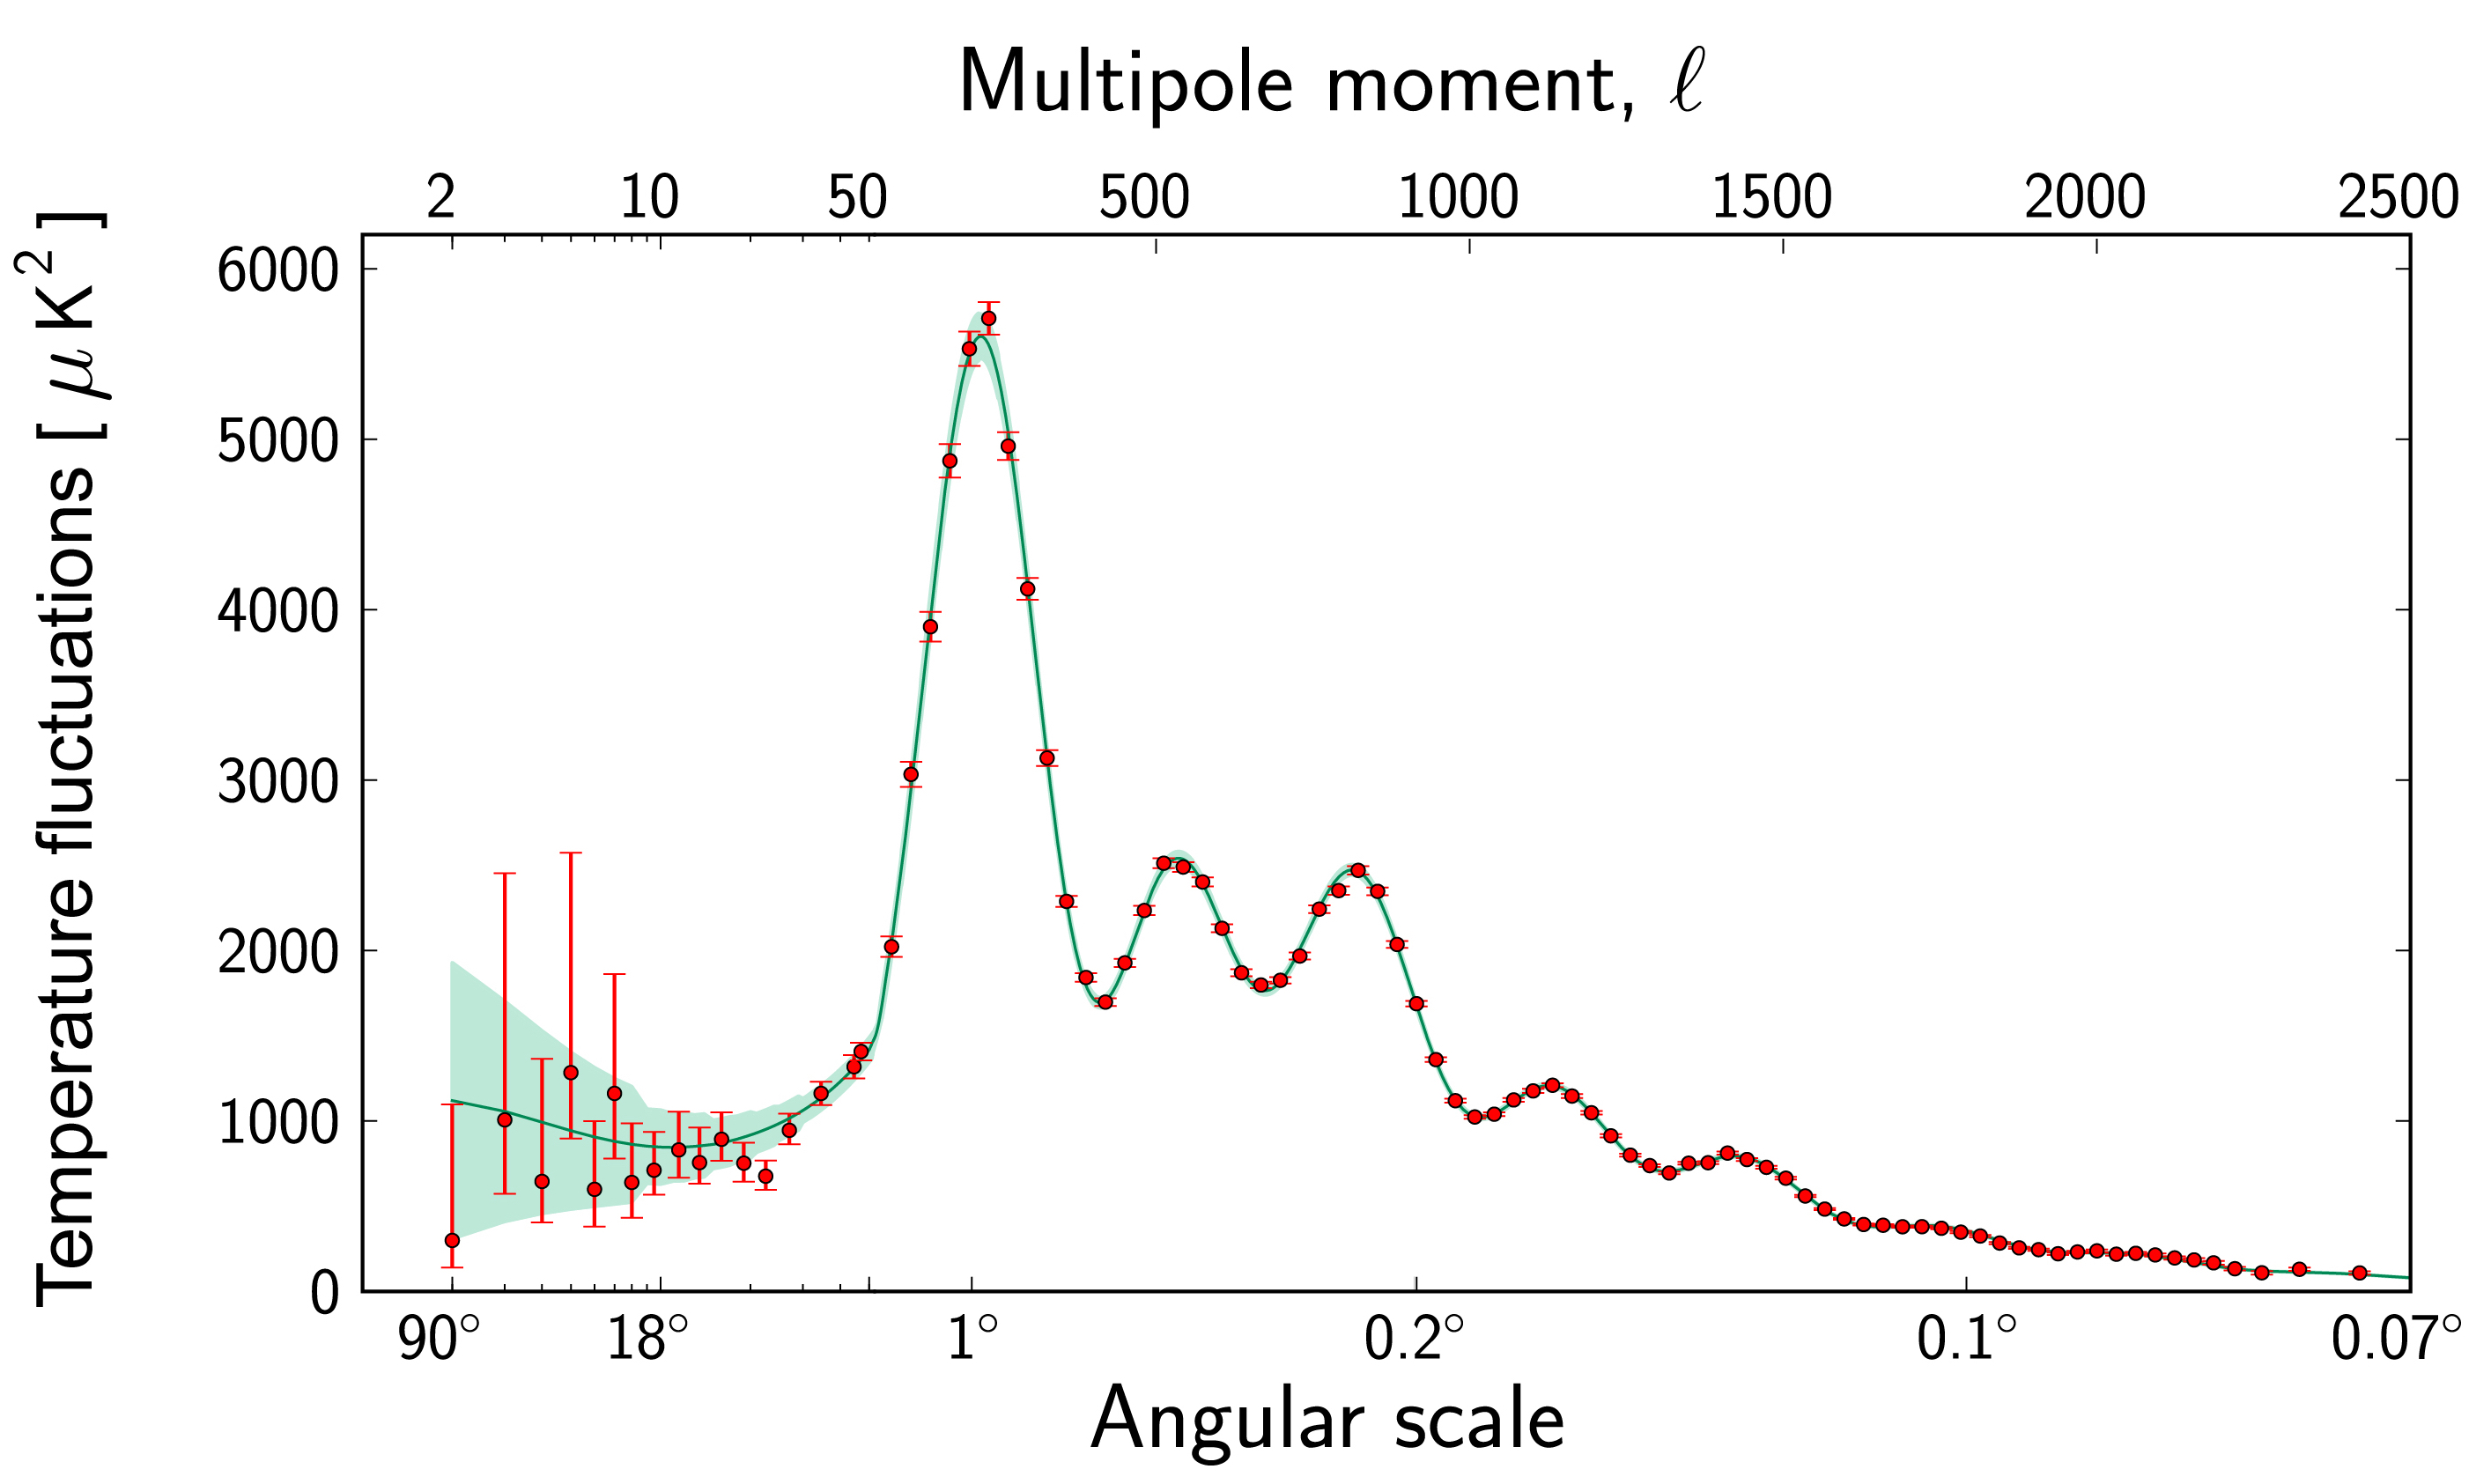
\includegraphics[scale=0.15]{Chapter_1/Figures/Planck_power_spectrum.jpg}
        \caption[The map of the all sky CMB radiation as illustrated by the Planck collaboration, showing in detail the temperature anisotropies.]%
        {The angular power spectrum of the CMB temperature fluctuations as measured by Planck. The green line fitted onto the seven acoustic peaks is the six-parameter $\Lambda$CDM model. The shaded area around the best-fit curve represents cosmic/sample variance, including the sky cut used.}
        \label{fig:cmb_power_spectrum}
        \end{center}
\end{figure}

The primary anisotropies of the CMB are due to the last scattering of photons in the recombination epoch. Perturbations in the primordial plasma lead to collapse of matter in regions of over-density. The gravitational collapse lead to an increase in radiation pressure of the photon-baryon plasma, which eventually counteracted local gravitational wells and set up acoustic oscillations. Photons from high-density regions at last scattering were redshifted climbing out of these potential wells. Furthermore, adiabatic fluctuations in these regions lead to an increase in temperature. and velocity fluctuations within the plasma would have further resulted in Doppler shifts in frequency. The peaks observed in the power spectrum correspond, roughly, to resonances in which the photons decouple when a particular mode is at its peak amplitude.

The ability to probe and image the very early universe via the CMB at the moment of recombination opens the way to understand, model and extract information about the contents of the early universe. The amplitudes and positions of the peaks observed in the power spectrum are dependent on the baryonic and non-baryonic matter content of the early universe, and on the geometry of space. Since light propagates along geodesics in space and the size of the horizon at recombination can be inferred by the properties of the plasma, the geometry of space can then be determined by the understanding of the the expansion history. A flat space-time corresponds to a first peak around $l$ of \sim220. The higher order peaks of the spectrum can provide information on the baryonic and non-baryonic matter densities in the early universe. In particular the third peak is sensitive to the density ratio of matter to radiation. The dampening observed as $l$ increased is due to the washing out of fluctuations initially set by inflation. The third peak, however is boosted relative to the rest, demonstrating the domination of matter in the plasma before the time of recombination and encapsulates the information present on the dark matter content of the early universe.

The power spectrum of the CMB is well described by the Lambda Cold Dark Matter ($\Lambda$CDM) model as shown in (\ref{fig:cmb_power_spectrum}). $\Lambda$CDM emerged as the standard model of cosmology in describing the evolution of the universe with its matter content \cite{Modern_Cosmology}. In explaining and parametrising the Big Bang cosmological model, $\Lambda$CDM requires a cosmological constant ($\Lambda$)---associated with the vacuum energy contribution or also known as dark energy, and the presence of ordinary and non-baryonic Cold Dark Matter (CDM). In fitting this model to the power spectrum, Planck extracts some of the density parameters defined in section (\ref{subsec:cosmological_principle}), where $\Omega_{\Lambda} =  0.6847 \pm 0.0073$ and $\Omega_{m} =  0.3153 \pm 0.0073$ \cite{Plank_2018, Plank_2018_2}. Furthermore, Planck extracts the baryon and cold dark matter densities from the $\Lambda$CDM model fit parameters to give $\Omega_{b}h^2 = 0.02237 \pm 0.00015$ and $\Omega_{c}h^2 = 0.1200 \pm 0.0012$. Normalising these with the the Hubble constant given in equation (\ref{eq:hubble_constant}) results in $\Omega_{b} \sim 0.049$ and $\Omega_{CDM} \sim 0.265$. The information captured by the CMB and its power spectrum points towards a universe that is \sim 68\% dark energy and \sim 32\% matter. The non-baryonic cold dark matter further contributes to \sim 84\% the total matter content of the universe.


\subsection{Big Bang Nucleosynthesis}
\label{subsec:BBN}

The radiation temperature of the universe moments after the big bang were above the MeV binding energies of nuclei and way above the KeV binding energies of atoms. Any nuclei or atom present would have quickly disintegrated into electrons, protons and neutrons. Within the first few minutes, when the temperatures dropped below nuclear binding energies, nuclear reactions lead to the formation of the very first nuclei via the process known as Big Bang Nucleosynthesis. The relative primordial abundance of isotopes such as D, $^{3}$He, $^{4}$He and $^{7}$Li synthesised minutes after the big bang and depend on the cosmological parameters of the universe \cite{pns}. 

As the baryon number is conserved at and below MeV temperatures, the process of nucleosynthesis and the abundance of primordial isotopes depend on the total baryon number and thus $\Omega_{b}$ in the early universe. The relative abundances can be measured today in places such as old stars, low mass local galaxies and the edges of distant galaxies, where a small change in primordial abundance is presumed. The primordial abundances of D, $^{3}$He, $^{4}$He and $^{7}$Li as predicted by the standard model of Big-Bang nucleosynthesis is shown in figure (\ref{fig:primordial_abundance}). The figure shows the theoretical dependency of primordial isotopic ratios on the baryon/photon ratio (\eta) in the early universe and by extension, on $\Omega_{b}$.

\begin{figure}[ht!]
    \begin{center}
        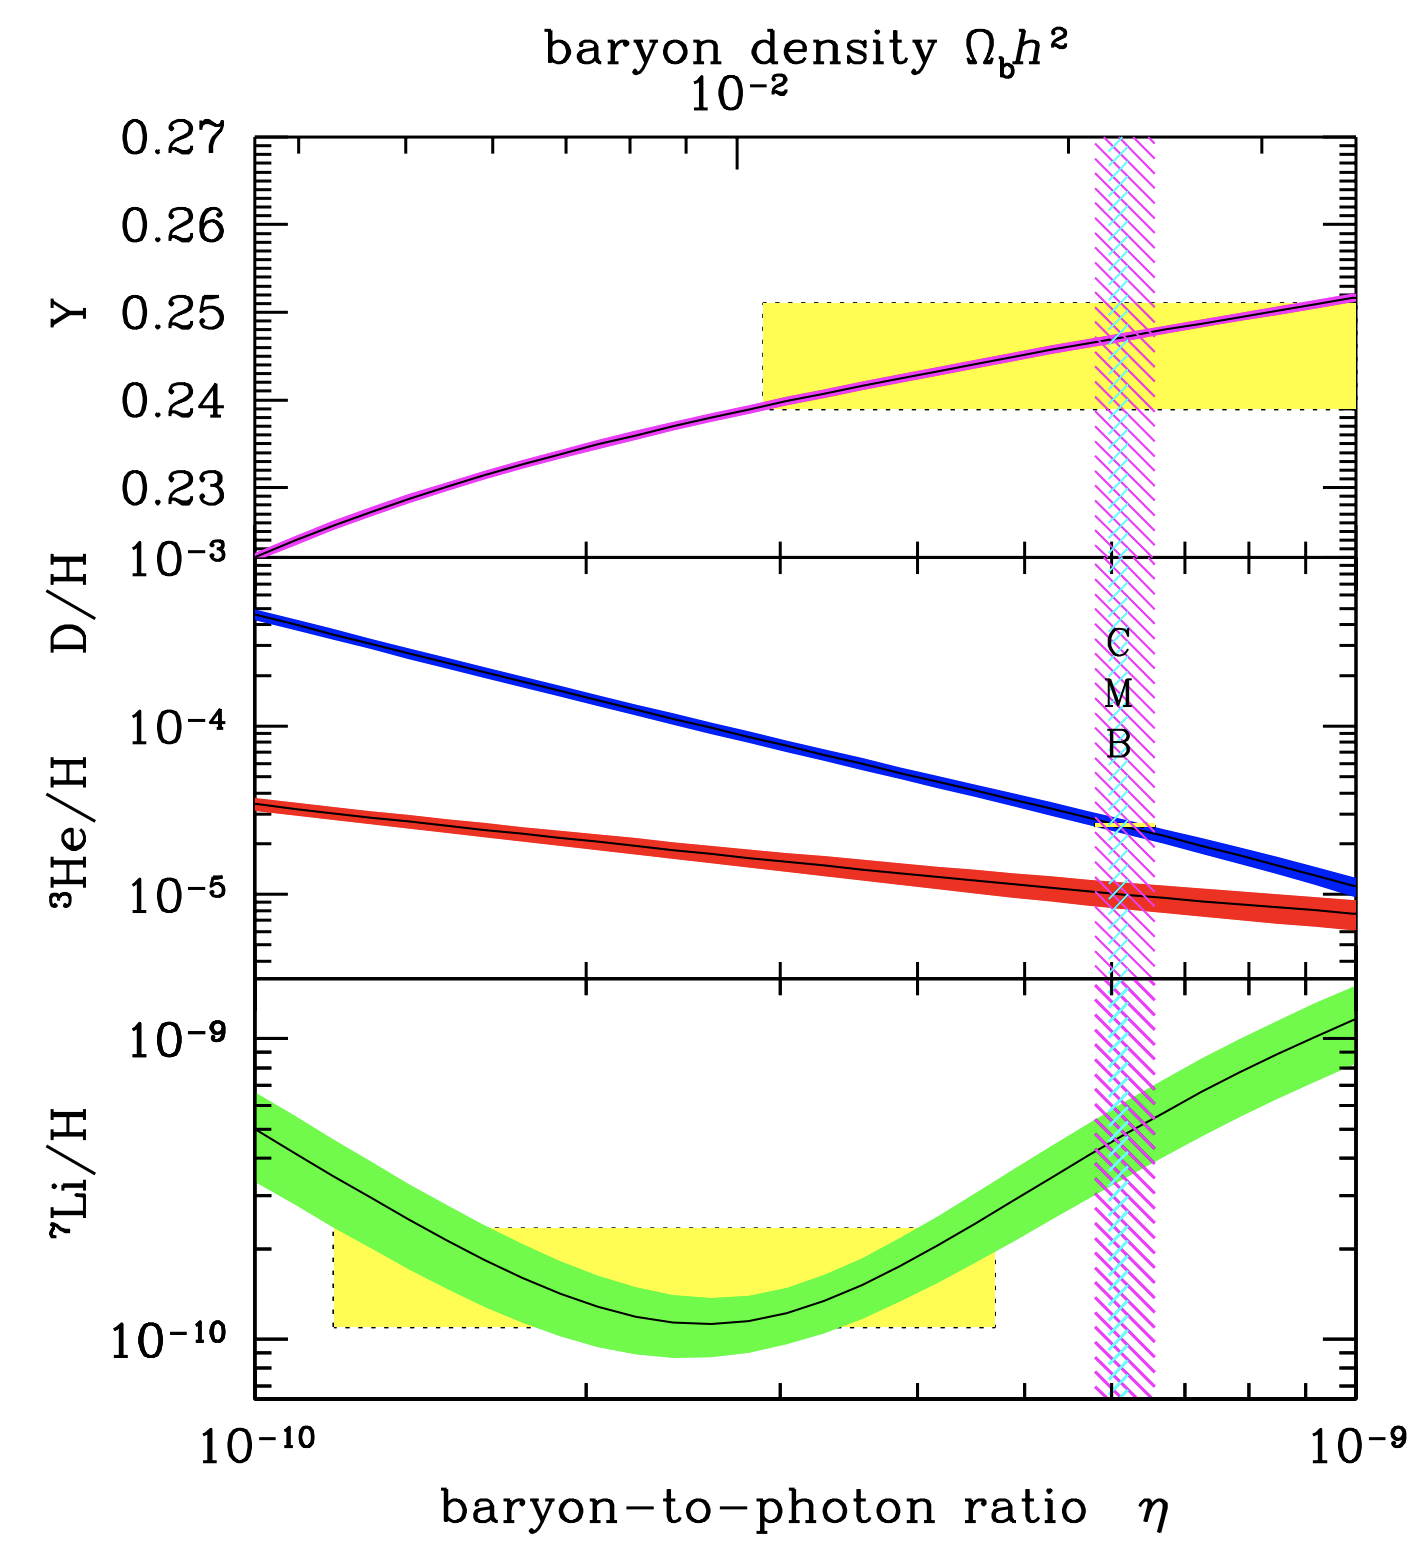
\includegraphics[scale=0.45]{Chapter_1/Figures/BBN_primordial_abundance.jpg}
        \caption[The primordial abundances of $^4$He, D, $^3$He, and $^7$Li as predicted by the standard model of Big-Bang nucleosynthesis]%
        {The primordial abundances of $^4$He, D, $^3$He, and $^7$Li as predicted by the standard model of Big-Bang nucleosynthesis with the bands highlighting the 95\% CL range. Yellow boxes indicate the observed light element abundances and the vertical band indicates the CMB measure of the cosmic baryon density \cite{BBN_figure}}.
        \label{fig:primordial_abundance}
        \end{center}
\end{figure}

Deuterium is usually entirely deployed when it is cycled into stars, and the only significant production mechanism is the process of BBN \cite{pns}. Hence, any detection of deuterium provides an upper limit on $\eta_{10}$ and lower limit on the ratio of D/H. The local interstellar value of D/H = $(1.56 \pm 0.40) \times 10^{−5}$ sets a limit of $\eta_{10} < 9$ \cite{d_h_measurements}. Although the \eta range measurements as illustrated by the boxes on figure (\ref{fig:primordial_abundance}) do not all overlap, they are all within a factor of \sim2 from each other. In particular, the discrepancy between the lithium abundance in comparison to the D/H and less-constraining $^4$He abundance is often referred to as the `lithium problem' and could simply reflect the difficulty in determining the primordial lithium abundance (discussed in detail here \cite{Fields_2011}). The measured D/H and $^4$He abundances are in great agreement when the lithium measurement is excluded in due to unknown systematic. The \eta range extracted from the more-precise measurement of D/H gives
%
\begin{equation}
    5.8 \; \leq \; \eta_{10} \; \leq \; 6.6 \; (95\% \; CL),
\end{equation}
%
which provides a measure for the baryon density of the universe as
%
\begin{equation}
    0.021 \; \leq \; \Omega_{b}h^2 \; \leq \; 0.024 \; (95\% \; CL).
\end{equation}
%
Despite the lithium problem, by using only well-established microphysics, the theoretical predictions of the BBN model is in good agreement with both the observations of the D/H abundance and with the baryon density parameter obtained from the CMB by Planck. As an independent observation to that of the CMB, measurements of the primordial isotopic abundances and the BBN model suggest that luminous baryonic matter density $\Omega_{lum} \simeq \Omega_{b}$. This can be seen as further evidence to that obtained from the CMB power spectrum and $\Lambda$CDM, suggesting that the total matter content of the universe cannot be explained by only the presence of baryonic matter alone and the matter density parameter $\Omega_{m} = \Omega_{b} + \Omega_{CDM}$, where a substantial degree of the mass density is comprised of cold dark matter. 

\subsection{Galaxy Rotation Curves}
\label{subsec:rotation_curves}

There is considerable cosmological evidence that most of the mass content of the universe is neither luminous matter nor radiation. Luckily, mass can be detected even if the constituents of this mass is `unseen'. The very early evidence for dark matter comes from studies in the early 1930s, where in studying galaxy cluster dynamics and applying the virial theorem to the coma cluster, Zwicky \cite{Fritz_Zwicky_1993} notice an unusual discrepancy between luminous mass and
estimated mass, making the first claim for unseen matter in galaxies. It wasn't until the 1960s when Ruben and Ford showed further evidence to support Zwicky's claims by studying the rotation curves of starts in spiral galaxies \cite{ruben_ford, ruben_ford_results}.

Galactic scale physics, such as the behaviour of stars orbiting spiral galaxy can readily be explained by Newtonian mechanics. Assuming spherical symmetry, the circular velocity $v_{circ}$ of stars or hydrogen gas clouds orbiting a spiral galaxy at a distance $r$ can be determined using a simple Newtonian relation
%
\begin{equation}
    v_{circ} = \sqrt{\frac{GM(r)}{r}},
\end{equation}
%
where G is the gravitational constant and $M(r)$ is the mass of the galaxy contained within $r$. The relationship above can be written in a form to give the total mass encapsulated up to a specific radius $M(r)$, if the velocities of stars at a distance $r$ can experimentally be obtained. For galaxies that are inclined to the line of sight, spectroscopic radial velocities and radio observations of the 21 cm line of neutral hydrogen at a number of positions on the galactic disc can be used to determine and map out the velocity rotation curves of such galaxies.

\begin{figure}[ht!]
    \begin{center}
        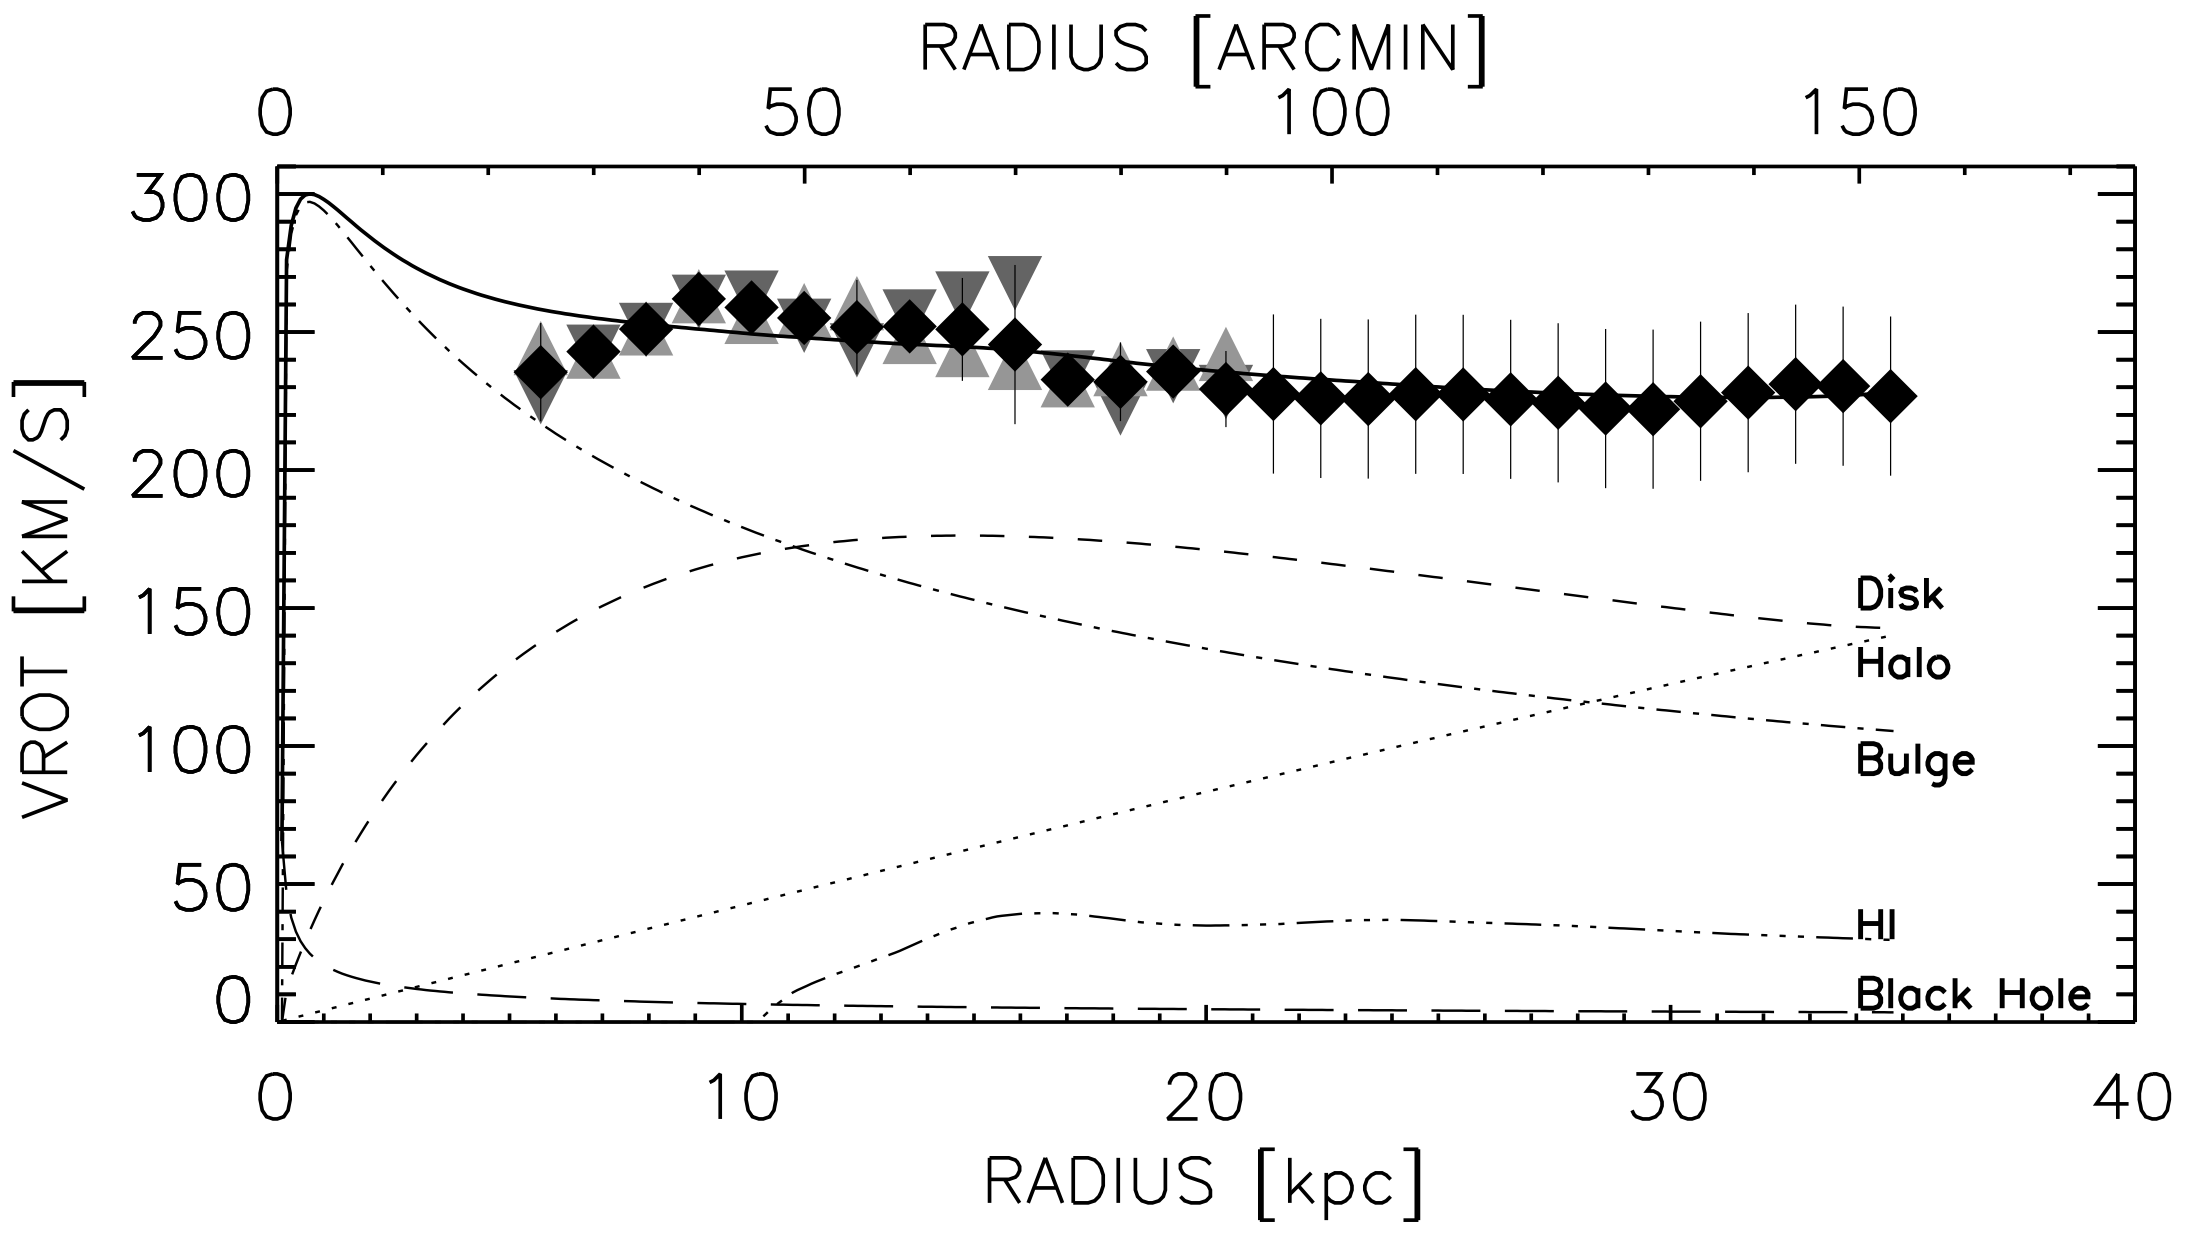
\includegraphics[scale=0.35]{Chapter_1/Figures/Rotation_curve_M31.jpg}
        \caption[Observed rotation curve and corresponding mass models for the Andromeda galaxy (M31) by using data from the Effelsberg and GBT 100 m observations.]%
        {The galactic rotation curve of the Andromeda galaxy (M31) as measured by the Effelsberg and GBT 100 m telescoped. The solid black line represents best fit to data and the corresponding lines below are models illustrating the sub-contributions from the galactic disk, dark matter halo and other factors as labeled on the plot \cite{Carignan_2006}.}
        \label{fig:rotation_m31}
        \end{center}
\end{figure}

The traditional view on the mass density of spirals galaxies implied that most of the mass would be contained within the central luminous region, as observed visibly, and rotational velocities measured beyond this point would be proportional to $1/r^2$. The observations presented in figure \ref{fig:rotation_m31}, show the rotation curve of the Andromeda galaxy (M31). The plot suggests that rotational velocities of M31 certainly is not proportional to $1/r^2$, but rather remains fairly constant after the central bulge ($\geq 10 \MathText{kpc}$). The constancy of rotational velocities can be explained by the addition of a dark matter halo into galaxies. If the dark matter halo were to extend way beyond the boundaries of the luminous bulge, this will result in rotation curves as shown for M31. A similar behavior to as seen in M31 has been observed in many other galaxies, including our own milky way \cite{Carignan_2006, Mr_z_2019}. Unless our understanding of gravity needs modification, as such proposed by MOND and other modified gravity theories (such as \cite{Milgrom_2015, Moffat_2006}), the overwhelming data from such galaxies indicate that dark matter halos can account for a significant proportion of the mass contained within galaxies. Combining these observations with those presented in previous sections, further indicate the need for non-baryonic matter in the Universe.



\subsection{Summary}
\label{subsec:evidence_summary}

The vast amount of observational data from different facets of cosmology and particle-astrophysics point towards a universe that is flat in geometry, and one which is comprised of dark energy, dark matter and ordinary matter---as presented in the standard model (SM) of particles. The primary evidence comes from the early universe physics encoded into the CMB, formation of primordial isotopes as demonstrated by BBN, galaxy dynamics and rotation curves and various other observations and realisations, such as large scale structure of of universe and the need for a form of dark matter to accommodate for the observed structure and galaxy formation \cite{LSS_coles}. In collating together our understanding of gravity, as outlined by General Relativity and the cosmological data presented, $\Lambda$CDM model of cosmology offers a framework which describes a universe with key cosmological parameters; $h_0 \; \sim0.674$, $\Omega_{\Lambda} \; \sim0.685$, $\Omega_{m} \; \sim0.315$  and $\Omega_{CDM} \; \sim0.265$. Our understanding of the particle content of the universe, as given by the SM of particle physics is insufficient in offering a candidate for the CDM content of the universe, leaving \sim 85\% of the matter content yet to be discovered.


%%------------------------------$$
\section{Dark Matter \& WIMPs}
\label{sec:candidates}

In an attempt to explain the discrepancy between $\Omega_{m}$ and $\Omega_{B}$, a vast number of hypothesis has been proposed. These models predominantly fall under three categories; dark matter explained via the introduction of new particles---stemming from beyond the standard model (BSM) physics, astrophysical objects, and by questioning the fundamentals of cosmology and gravity and explaining DM by alternative gravity models. However, the most promising is Weakly Interacting Massive Particles (WIMPs). 

\subsection{Non-WIMP Dark Matter Candidates}
\label{subsec:non_wimp_dm}

\subsubsection{Axions}
\label{subsubsec:axions}

The axion is a pseudo-Nambu-Goldstone boson, proposed by the Peccei–Quinn theory as an extension to the QCD Lagrangian in the SM to solve the strong Charge-Parity (CP) problem \cite{axions_cp}. The QCD Lagrangian is given as
%
\begin{equation}
    \mathcal{L}_{QCD} = -\frac{1}{4}G^{a}_{\mu\nu}G^{a\mu\nu} + \sum_{n}^{j=1} \left[ \bar{q}_{j}\gamma{}^{\mu}iD_{\mu}q_{j} - (m_{j}q^{\dagger}_{Lj}q_{Rj} + h.c.)  \right] + \frac{\theta{}g^{2}}{32\pi{}^{2}}G^{a}_{\mu\nu}\Tilde{G}^{a\mu\nu},
\end{equation}
%
where the CP violating term $\mathcal{L}_{\theta} = \Bar{\theta} (\alpha_{s}/8\pi)G^{a}_{\mu\nu}\Tilde{G}^{a\mu\nu}$, in which $-\pi \leq \Bar{\theta} \leq +\pi$ is the effective $\Bar{\theta}$ parameter after diagonalising quark masses. Although the last term of the Lagrangian does not contribute in perturbation theory, it does however contribute through non-pertubative effects, associated with QCD instantons \cite{Sch_fer_1998}. The QCD Lagrangian contains terms that may lead to CP violation in scenario where none of the quark masses vanish, leading to a non-zero \theta dependence \cite{gauge_theory_vacuum, tHooft:1976rip}. If $\Bar{\theta} \neq 0$, then QCD violates both Parity (P) and CP symmetry. However, the presence of CP violation in QCD leads to an electric dipole moment (EDM) of the neutron. The experimental bounds placed by neutron EDM experiments currently suggest an absence of CP violation in strong interactions, yielding an upper limit of $\Bar{\theta} \leq 10^{-10}$, where $\Bar{\theta} = \mathcal{O}(1)$ is otherwise completely satisfactory \cite{edm_limit}. The question then is: given that $\Bar{\theta}$ take any value between $-\pi$ and $\pi$, why then is $\Bar{\theta}$ so close to zero? This presents a naturalness problem for SM, where the fine-tuning required here is presented as the strong CP problem of QCD.

The spontaneously broken global Peccei-Quinn $U_{PQ}(1)$ symmetry was introduced to solve the strong CP problem \cite{axions_cp}. The axion is the pseudo-Nambu-Goldstone boson associated with the spontaneous breaking of the $U_{PQ}(1)$ symmetry. This symmetry is broken due to the anomalous triangle coupling of the axions to the gluons, 

%
\begin{equation}
    \mathcal{L}_{\theta} = \left( \frac{\phi_A}{f_{A}} - \Bar{\theta} \right) \frac{\alpha_{s}}{8\pi} G^{a}_{\mu\nu}\Tilde{G}^{a\mu\nu},
\end{equation}
%
where $\phi_{A}$ is the axion field and $f_{A}=v_{a}N$ the axion decay constant; $v_{a}$ is the vacuum expectation value of the spontaneously broken $U_{PQ}(1)$ and $N$ is and integer normalisation factor expressing the colour anomaly of $U_{PQ}(1)$. The introduction of this new symmetry results in the induction of a potential $\phi_{A}$ from the non-perturbative fluctuations of the gluon fields, whose minimum is at $\phi_{A} = \Bar{\theta}f_{A}$, thereby canceling the $\Bar{\theta}$ terms in the QCD Lagrangian and restoring CP symmetry. 





\subsubsection{Neutrinos}
\label{subsubsec:neutrinos}



\subsection{WIMPs}
\label{subsec:wimp_dm}




%%------------------------------$$
\section{Direct Detection}
\label{sec:candidates}